\chapter{Introduction}
Air pollution is caused by different typologies of gas pollutants that are present in the first meters (< 150 m) of the atmosphere and cause therefore damages to humans and environment. As air pollution is becoming the largest environmental health risk, the monitoring of air quality has drawn much attention in both laboratory studies and specific field tests and data collection campaigns. Government agencies and local administrations have, generally, provided and used monitoring stations on dedicated sites in cities and urban areas. Usually the studies have been conducted using fixed stations that are very reliable but produce only coarse-grained 2D monitoring, with several kilometers between two monitoring stations; or the stations monitor the same local area for long periods.
Other approaches show that applications using simple system of sensors have been developed to monitor the fine-grained air quality using densely deployed sensors \cite{8718193}\cite{8682518}. In any case, the fixed sensor station may achieve high precision, but have high cost and require maintenance and suffer especially for lack of mobility.
Furthermore, these approaches don't account for the vertical gradients of air pollution levels. As shown in research \cite{wu2014mapping}\cite{neuberger1954vertical} the concentrations of air pollutants can vary greatly at different heights and this is a sensitive factor in circumstances such as buildings in urban areas and possible polluting plants in industrial areas.
The usage of Unmanned Aerial Vehicles (UAVs) has been particularly rich in the latest years due to their flexibility, mobility and affordable cost. Current monitoring systems are not able to satisfy every need of modern cities and industrial areas and UAVs are valuable supporting elements in this scenario.
In terms of urban conditions, which is the main subject of the present study, UAVs can be used to measure environmental parameters such as illumination, wind speed, temperature, humidity, air quality and much more. In any case, for a complete analysis, both ground sensing and aerial sensing are necessary to provide 3D mapping and gas profiling. In our ARIA project, we equipped with the same set of sensors the devices that execute sensing on the ground, and the systems that execute aerial sensing on board the \gls{uavs}, which we are deploying in vertical swarms, to measure pollution levels at different heights.
The fixed ground sensing suite is able to collect data in a continuous way, but the air quality of the higher levels of air off the ground cannot be detected, so the contemporary use of drones is mandatory. Aerial sensing, on the contrary, is able to sense the air quality off the ground, but it cannot be executed for very long periods due to the high consumption of battery power and human time. By merging the potentialities of these two systems of sensing suites, a better set of data can be collected. A trade off on the possible sensors and UAVs has been performed and quadcopters are the preferred platform for monitoring because of their simplicity, low cost and hovering capabilities. On the contrary a possible bias of data is due to the the influence of air jets created by the rotor rotation or by the electromagnetic field generated by the antennas present on board. The problem of choosing the best location of the sensors is examined in \cite{8453584} based on the physical structure of the drones. Our approach is to use an extension on which we fix the sensors in order to suck the air away of the main air jets.
\section{Related works and state of the art}
\subsection{Air Pollution}
According to \cite{epc} "Air pollution can be defined as the presence of toxic chemicals or compounds (including those of biological origin) in the air, at levels that pose a health risk. In an even broader sense, air pollution means the presence of chemicals or compounds in the air which are usually not present and which lower the quality of the air or cause detrimental changes to the quality of life (such as the damaging of the ozone layer or causing global warming)".
Air pollution is extremely complex to evaluate and there are many polluting substances in the atmosphere. The \gls{epa} (of United States) takes these 6 (the "criteria air pollutants") in consideration in its studies:
\begin{table}[h!]
\caption{Criteria air pollutants and their health effects \cite{7946542}}
\centering
\begin{tabular}{ |c|c|c|c| }
    \hline
    \thead{Chemical symbol} & \thead{Substance} & \thead{Characteristics} & \thead{Effect} \\ [0.5ex]
    \hline
    \hline
    CO & Carobon Monoxide & Colorless, odorless gas & \makecell{Reducing oxygen delivery to the \\ body's orogans and tissues} \\
    \hline
    $NO_2$ & Nitrogen Dioxide & Highly reactive gas & \makecell{Risk of emphysema, asthma \\ and bronchitis diseases} \\
    \hline
    $O_3$ & Ozone & Pale blue gas & \makecell{Chest pain, coughing, \\ throat irritation} \\
    \hline
    $SO_2$ & Sulfur Dioxide & Colorless, irritating smell gas & \makecell{Risks of bronchoconstriction \\ and increase of asthma symptoms} \\
    \hline
    $PM_{2.5}$ and $PM_{10}$ & Particulate Matter & Inhalable particles & \makecell{Premature death and respiratory \\ symptoms} \\
    \hline
    Pb & Lead & Metal particles & \makecell{Accumulate in bones and \\ affecting the nervous system} \\ [1ex]
    \hline
\end{tabular}
\label{table:airpollutants}
\end{table}
\subsection{Air quality monitoring}
Air quality monitoring is an essential part in order to know what measures to put in place \cite{who-airquality} to protect our health and the environment, which are strongly connected.
In the Veneto region, Italy, the area of this study, the ARPAV\cite{arpav} has put in place a conventional monitoring network to track major air pollutants and enforce restrictory measures on polluting factors (such as transportation) if necessary. Figure \ref{fig:arpav-map} shows the map of ARPAV's current 2D monitoring network, which gives an example of the very low spacial resolution of conventional air quality monitoring systems.
\begin{figure}[h!]
    \centering
    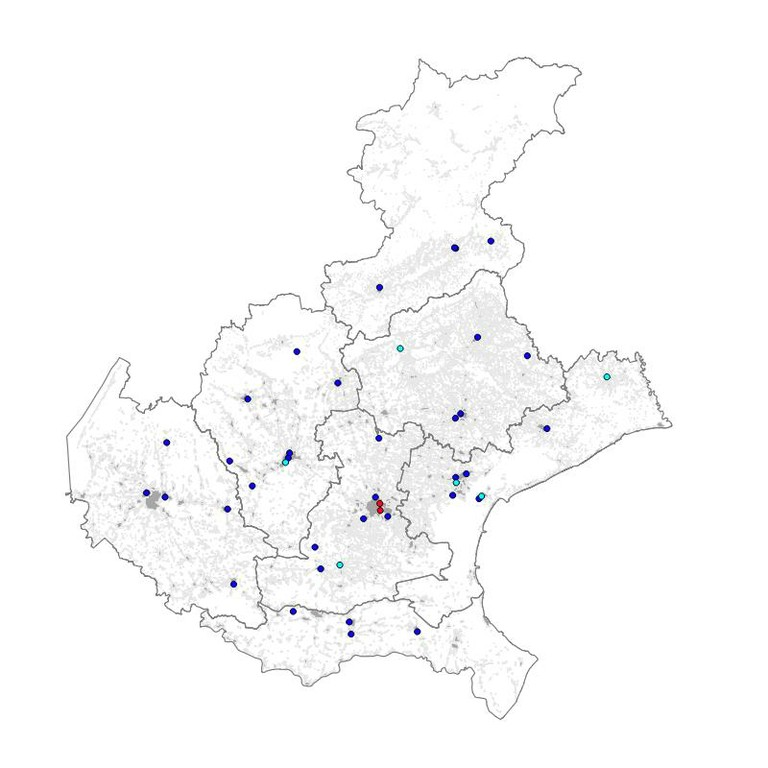
\includegraphics[width=0.7\textwidth]{images/ARPAV stazioni rete 2019.jpg}
    \caption{ARPAV monitoring netowrk in the Veneto region, Italy\cite{arpav}}
    \label{fig:arpav-map}
\end{figure}
\subsection{Low-cost sensors}
The \gls{epa} also provides the Air Sensor Guidebook\cite{williams2014air} which gives extensive information on air quality and low-cost sensors. Due to their prohibitive cost and complexity, conventional air pollution monitoring systems have low spacial and temporal resolution. Low-cost sensors, instead, can be deployed more diffusely with high spacial and temporal resolution, while trading most of their accuracy. They are, in fact, heavily influenced by many factors, especially temperature, humidity, wind and presence of other gases in the air.  Due to their lightweight, only low-cost sensors can be mounted on drones: the aforementioned influence factors could introduce even more inaccuracy, especially wind generated from the rotors.
\cite{s151229859} among other things presents an evaluation of air quality sensors classifying their performances by the most important parameters.
\subsection{Drone systems}
Coordinating data collection and movements is quite hard, considering the low computational power of UAVs, the inaccuracy of GPS and the general wireless communication issues. \cite{s151229859} is a survey on the communication issues releted to drone networks. The energy constraint is really impactful on long missions and poses a major limitation to the spreading of drone technology. Drones have excellent mobility and data gathering prowess, but cannot always rely on coming back to the base to deliver their information. Implementing reasonable communication protocols and algorithms is necessary to improve efficiency. 
\subsection{Drone monitoring and sensing}
Thanks to their mobility and flying movement, drone monitoring and sensing capabiliteis are very valuable. In urban settings \gls{uavs} can monitor noise, traffic, light, wind, temperature, humidity, air quality and many other parameters.
As shown earlier, conventional air quality monitoring systems have very low spatial and temporal resolution. \gls{uavs} based systems could measure specific areas with great convenience and felxibility and hybrid ground and air based solutions could routinely track the air pollution levels of parts of a city. A single UAV, however, is very limited in its performance due to its coverage, energy autonomy and small selection of sensors.  Swarms, instead, can provide full coverage of an area, while coordinating the best routes to visit each sensing node. Equipping different drones with different sensors is far easier and more flexible than having one doing everything on its own.
\cite{7946542}, \cite{evangelatos2015airborne}, \cite{8675167}, \cite{8662050} propose different solutions for a \gls{wsn} using \gls{uavs}. \cite{8675167} in particular examines an application in smart cities, where a hybrid ground and air based system tracks an urban area.
\section{Dissertation structure}
This dissertation describes the \gls{aria} project solution for the monitoring of air pollution. It is divided into 6 chapters:
\begin{itemize}
    \item Chapter 1 describes the introduction, an overview on the topic of air pollution, the motivation to approach the problem, the motivation of the proposed solution, related works, the state of the art and the dissertation objective.
    \item Chapter 2 describes the system architecture, that is the \gls{uavs} that are being used, their design, specifications and functionality.
    \item Chapter 3 describes the sensor payload, the motivation of the adopted sensors and their use.
    \item Chapter 4 describes the software implementation for the data collection of the sensors and the communication of the \gls{uavs}.
    \item Chapter 5 shows the results of a test flight using the proposed solution.
    \item Chapter 6 presents what conclusions can be taken after all the developed work, and what improvements can be done in the future.
\end{itemize}
\section{Dissertation objective}
The objective of this dissertation is to describe the solution proposed by the \gls{aria} project for air pollution monitoring, in particular the software impelementation, to show preliminary results and discuss their revelance in future applications.